\documentclass[aps,pra,twocolumn,showpacs,superscriptaddress,floatfix,10pt]{revtex4}
\usepackage{graphicx}
\usepackage{psfrag}
\usepackage{amssymb,amsmath}
\usepackage{physics}
\usepackage{float}
\usepackage{dsfont}
\usepackage{algorithmicx}
\usepackage[noend]{algpseudocode}
%\usepackage[dvips]{color}
\algdef{SE}[DOWHILE]{Do}{doWhile}{\algorithmicdo}[1]{\algorithmicwhile\ #1}%

%\setlength{\topmargin}{0.1cm}
\begin{document}
\newcommand{\beq}{\begin{equation}}
\newcommand{\eeq}{\end{equation}}
\newcommand{\ben}{\begin{eqnarray}}
\newcommand{\een}{\end{eqnarray}}
\newcommand{\bea}{\begin{array}}
\newcommand{\eea}{\end{array}}
\newcommand{\om}{(\omega )}
\newcommand{\bef}{\begin{figure}}
\newcommand{\eef}{\end{figure}}
\newcommand{\leg}[1]{\caption{\protect\rm{\protect\footnotesize{#1}}}}
\newcommand{\ew}[1]{\langle{#1}\rangle}
\newcommand{\be}[1]{\mid\!{#1}\!\mid}
\newcommand{\no}{\nonumber}
\newcommand{\etal}{{\em et~al }}
\newcommand{\geff}{g_{\mbox{\it{\scriptsize{eff}}}}}
\newcommand{\da}[1]{{#1}^\dagger}
\newcommand{\cf}{{\it cf.\/}\ }
\newcommand{\ie}{{\it i.e.\/}\ }   

\newcommand{\spazio}{\vspace{0.3cm}}%{\vspace{1.05cm}}
\hyphenation{bio-mol-ecules}
\newcommand{\de}[1]{\frac{\partial}{\partial{#1}}}
\newcommand{\U}{\tilde{U}}
\newcommand{\V}{\tilde{V}}


\title{Approaching near-perfect state discrimination of photonic Bell states through the use of Ancillas}

\author{Jake~A.~Smith}
\affiliation{Tulane University, Department of Physics, New Orleans, Louisiana 70118, USA}

\author{Lev Kaplan}
\affiliation{Tulane University, Department of Physics, New Orleans, Louisiana 70118, USA}

 \begin{abstract}
 	Finish the experiment first before writing abstract.
\end{abstract}                                                               
\date{\today}
\pacs{***}
\maketitle
\section{Introduction}
\label{Intro}
In quantum information processing, the ability to perform proper measurements is imperative. Because of the effects of observation on superposition and entanglement, there is a fundamental difference between measurement at a quantum and macroscopic level. As a result, implementation of a quantum measurement can be non-trivial. In the linear optical quantum computing paradigm, even a seemingly simple Bell measurement has presented significant challenge. This is a problem; Bell state discrimination plays an important role in teleportation, which is a basic building-block for many quantum algorithms. Here, we attempt to use numerical techniques to design an efficient photonic Bell state analyzer using only deterministic linear optics and ancilla resources. 

We can encode qubits into the polarization or spatial states of a single photon. Then, the Bell states are represented by a maximally entangled EPR pair of photons. In the Fock basis, this ensemble is written
\begin{eqnarray}
\label{Bell States Creation Operator 1}
\ket{\phi_1} = \frac{1}{\sqrt{2}} (\hat{a}_1^\dagger \hat{a}_3^\dagger + \hat{a}_2^\dagger \hat{a}_4^\dagger) \ket{0} \\
\label{Bell States Creation Operator 2}
\ket{\phi_2} = \frac{1}{\sqrt{2}} (\hat{a}_1^\dagger \hat{a}_3^\dagger - \hat{a}_2^\dagger \hat{a}_4^\dagger) \ket{0} \\
\label{Bell States Creation Operator 3}
\ket{\phi_3} = \frac{1}{\sqrt{2}} (\hat{a}_1^\dagger \hat{a}_4^\dagger + \hat{a}_2^\dagger \hat{a}_3^\dagger) \ket{0} \\
\label{Bell States Creation Operator 4}
\ket{\phi_4} = \frac{1}{\sqrt{2}} (\hat{a}_1^\dagger \hat{a}_4^\dagger - \hat{a}_2^\dagger \hat{a}_3^\dagger) \ket{0} \\
%\ket{\psi_1} = \frac{1}{\sqrt{2}} \ket{1,0,1,0} + \frac{1}{\sqrt{2}} \ket{0,1,0,1} \\
%\ket{\psi_2} = \frac{1}{\sqrt{2}} \ket{1,0,1,0} - \frac{1}{\sqrt{2}} \ket{0,1,0,1} \\
%\ket{\psi_3} = \frac{1}{\sqrt{2}} \ket{1,0,0,1} + \frac{1}{\sqrt{2}} \ket{0,1,1,0} \\
%\ket{\psi_4} = \frac{1}{\sqrt{2}} \ket{1,0,0,1} - \frac{1}{\sqrt{2}} \ket{0,1,1,0} \\
\label{Bell State Ensemble}
\rho = \frac{1}{4} \sum_{x=1}^{4} \outerproduct{\phi_x}{\phi_x}. \quad  \enspace
\end{eqnarray}
The action of a linear optical quantum circuit on an optical state can generally be described by the transformation of creation operators~\cite{Reck}:
\begin{equation}
\label{LO Creation Operator Transformation}
\hat{a}^\dagger_\alpha \rightarrow \sum_{\beta=1}^{M} U_{\alpha\beta} \hat{a}^\dagger_\beta
\end{equation}
where $U_{\alpha \beta}$ are the elements of some unitary complex matrix $U$ and $M$ is the total integer number of optical modes. As it turns out, we cannot implement a perfect von Neumann measurement in applying Eq.~(\ref{LO Creation Operator Transformation}) to Eq.~(\ref{Bell States Creation Operator 1}-\ref{Bell States Creation Operator 4}). Formally, there exists no unitary matrix $U$ such that using perfect photon-number resolving detectors at each of the four circuit output modes allows a perfectly unambiguous measurement; at least two of the Bell states will always be indistinguishable. The crux of the problem is that linearly accessible entangling operations between photons allowed by Eq.~(\ref{LO Creation Operator Transformation}) are severely restricted to bosonic interference~\cite{Review Paper} and we are thus unable rotate the Bell states into non-overlapping Fock spaces for a photo-counting measurement. In 2001, the KLM~\cite{KLM,KLM2} scheme for implementing a CNOT gate between two qubits encoded in the in the dual rail~\cite{Review Paper} demonstrated that incorporating probabilistic partial measurements and ancilla resources into linear optical circuits allowed a new profitable set of transformations beyond those of Eq.~(\ref{LO Creation Operator Transformation}). 

Unfortunately, a series of "no-go" theorems on optical state discrimination seemed to limit the benefit of using these extra tools in a Bell state analyzer. First, it was demonstrated by L\"utkenhaus and Calsamiglia that a completely perfect measurement on an ensemble of Bell states using only linear components, multistage partial measurements and ancilla resources cannot exist~\cite{Lutkenhaus}. This theorem was later extended by~\cite{Carollo}; we apparently cannot implement a perfect measurement using these tools on \textit{any} set of indistinguishable orthonormal Fock states. Further, in the subclass of tools using only vacuum ancilla modes, it was shown that an analyzer cannot perfectly distinguish equi-probable Bell states (the ensemble in Eq.~(\ref{Bell State Ensemble})) more than half of the time~\cite{Calsamiglia}. However, it was shown by~\cite{Ewert} that this upper bound is lifted if we don't restrict our ancilla modes to be vacuum.

These no-go theorems are, however, somewhat complicated by the fact that they don't provide an exact upper bound on distinguishability. A "perfect" measurement is a meaningless limit in the real world and an arbitrarily close-to-perfect measurement would be  equally as invaluable for practical applications in quantum information processing. In 2011,~\cite{Pavicic} presented a scheme for near-perfect Bell state discrimination, though this paper was later retracted. This is clearly a difficult problem with no easy solutions.

Here, we use computational techniques to find a clear trend in linear improvement to Bell state measurements using only ancilla photons and vacuum modes (we find using multistage measurements to be ineffectual). Extrapolating these results, we apply analytic techniques to learn what we can about effective linear optical analyzers. We've made some progress, which may be of use to others who are working on this problem.
\section{Transforming the Bell states}
An optical quantum state can be written as a complex vector
\begin{equation}
\label{LO State Fock Vec Basis}
\ket{\psi} = \sum_{\vec{n}} c_{\vec{n}} \ket{\vec{n}} \,
\end{equation}
where
\begin{equation}
\ket{\vec{n}} = \ket{n_1,n_2,\dots,n_M}
\end{equation}
are the Fock states. A general linear optical transformation described by Eq.~(\ref{LO Creation Operator Transformation}) can also be written in the form of a linear operator $\hat{A}(U)$,
\begin{equation}
	\ket{\psi^\prime} = \hat{A}(U) \ket{\psi}.
\end{equation}
We define
\begin{equation}
\label{m definition}
\ket{\vec{m}} = \ket{m_1,m_2,\dots,m_N}
\end{equation}
where $m_\alpha$ is the mode-location of photon number $\alpha$ and $N$ is the total number of photons in the system. Of course the choice of vector $\ket{\vec{m}}$ for a given $\ket{\vec{n}}$ is not unique, since photons are indistinguishable and labeling them is an arbitrary process. We simply need to choose \textit{some} labeling and pick any valid $\ket{\vec{m}}$ for each $\ket{\vec{n}}$. Then the elements of the matrix representation of $\hat{A}(U)$ in the basis $\outerproduct{\vec{n}^\prime}{\vec{n}}$ are given by
\begin{eqnarray}
\label{A_U}
A(U)_{\vec{n}^\prime,\vec{n}} = \quad \quad \quad \quad \quad \quad \quad \quad \quad \quad \quad \quad \quad \quad \quad \quad \quad \\ \small \nonumber \prod_{p=1}^{M} \frac{\sqrt{n_p^\prime !}}{\sqrt{n_p !}} \left[\sum_{\textrm{perm}(\vec{m}^\prime)} U_{m_1 m_1^\prime} U_{m_2 m_2^\prime} \dots U_{m_N m_N^\prime} \right] \,,
\end{eqnarray}
where the summation is over all distinct permutations of integer entries in the vector $\vec{m}^\prime$. For proof of Eq.~(\ref{A_U}), see~\cite{Jake Smith}.

Here, we allow the use of $N_a$ integer number of ancilla photons and define our Bell states in the Fock ($\ket{\vec{n}}$) basis
\begin{equation}
\label{Bell States Phi}
	\ket{\psi_x} = \ket{1,1,\dots,1_{N_a}} \otimes \ket{\phi_x}
\end{equation}
e.g. the first Bell state is
\begin{eqnarray}
	\ket{\psi_1} = \frac{1}{\sqrt{2}}  \ket{1,1,\dots,1_{N_a},1,0,1,0} \\
	+ \frac{1}{\sqrt{2}} \ket{1,1,\dots,1_{N_a},0,1,0,1}. \nonumber 
\end{eqnarray}
The reader should note the total number of photons and modes are now
\begin{eqnarray}
	& N = N_a + 2 \\
	& M = N_a + 4.
\end{eqnarray}
We allow a standard von Neumann measurement; Alice chooses one of the Bell states $\ket{\psi_x}$ and sends it to Bob who runs the state through his analyzer $U$ and performs a photon-counting measurement at every output mode.
If Alice sends Bell state $\ket{\psi_x}$, the probability Bob measures state $\ket{\vec{n}^y}$ is
\begin{equation}
	\label{Probability of Measurment}
	p( y | x ) = \abs{\bra{\vec{n}^y} \hat{A}(U) \ket{\psi_x}}^2 \, .
\end{equation}
\section{The Classical Mutual Information}
\label{Section on Mutual Entropy}
To gauge the success of Bob's measurement device, we choose the classical mutual information, $H(X:Y)$. This quantity is bound from above by Holevo's theorem which is
given by
\begin{equation}
\label{Holevo Theorem}
H(X:Y) \le S(\rho) \le H(X).
\end{equation}
where $S(\rho)$ is the von Neumann entropy of a quantum ensemble and $H(X)$ is the classical Shannon entropy.
For the ensemble defined in Eq.~(\ref{Bell State Ensemble}), these quantities are both fixed;
\begin{equation}
	S(\rho) = H(X) = \mbox{2 bits}.
\end{equation}
The higher the mutual entropy, the better Bob was able to distinguish the Bell states. We say a Bell analyzer is near-perfect if
\begin{equation}
	\label{Near Perfect Condition}
	H(X:Y) = \lim\limits_{\epsilon \rightarrow 0} (2 - \epsilon) \mbox{ bits.}
\end{equation}
Formally, we define
\begin{equation}
	\label{Mutual Entropy}
	H(X:Y) = H(X) - H(X|Y)
\end{equation}
where $H(X|Y)$ is the conditional information
\begin{equation}
\label{Conditional Entropy}
\small
H(X|Y) = \frac{1}{4} \sum_{y \in Y} \sum_{x \in X} p(y|x) \log_2 \frac{\sum_{x^\prime} p(y|x^\prime)}{p(y|x)}\,.
\end{equation}
\section{Numerical Minimization of the conditional information}
\label{Section on Numerical Minimization}
To test the capability of a linear optical Bell state analyzer, we can numerically minimize Eq.~(\ref{Conditional Entropy}) over the circuit design $U$. In general, $U$ is constrained to be unitary. Here, however, we find minimization convergence is improved if we allow $U$ to be \textit{sub-unitary}, meaning $U$ can be any complex matrix such that the singular values all satisfy $\lambda \le 1$. This is equivalent to allowing vacuum modes outside the space of our measurement modes on which we do not perform any measurement. We call these modes the garbage modes and need to add a term to Eq.~(\ref{Conditional Entropy}) to accommodate them
\begin{equation}
\label{Condition Information with Garbage modes}
\small	\tilde{H}(X|Y) = H(X|Y) + \sum_{x \in X} \tilde{p}(y|x) \log_2 \frac{\sum_{x^\prime} \tilde{p}(y|x^\prime)}{\tilde{p}(y|x)}\,
\end{equation}
where
\begin{equation}
	\tilde{p}(y|x) = 1 - \sum_{y \in Y} p(y|x).
\end{equation}
In other words, all measurement outcomes in which photons have leaked into the garbage modes are consolidated into one.

We set $U$ to a general singular value decomposition,
\begin{equation}
	\label{Singular Value Decomposition}
	U = V D W
\end{equation}
where
\begin{eqnarray}
	& V = e^{i \tilde{V}} \\
	& W = e^{i \tilde{W}} \\
	& D =  \begin{pmatrix} e^{-\lambda^2_1} & 0 & 0 & \hdots & 0 \\ 0 & e^{-\lambda^2_2} & 0 & \hdots & 0 \\ 0 & 0 & e^{-\lambda^2_3} & \hdots & 0 \\ \vdots
	& \vdots & \vdots & \ddots & \vdots \\
	0 & 0 & 0 & \hdots & e^{-\lambda^2_M} \end{pmatrix} 
\end{eqnarray}
and minimize Eq.~(\ref{Condition Information with Garbage modes}) over all hermitian matrices $\tilde{V}$, $\tilde{W}$ and real numbers $\{\lambda_k\}$ using a quasi-Newton method without any constraints. Results are presented in Fig.~(\ref{Mutual Information Results}).
\begin{figure}[ht]
	\centering
	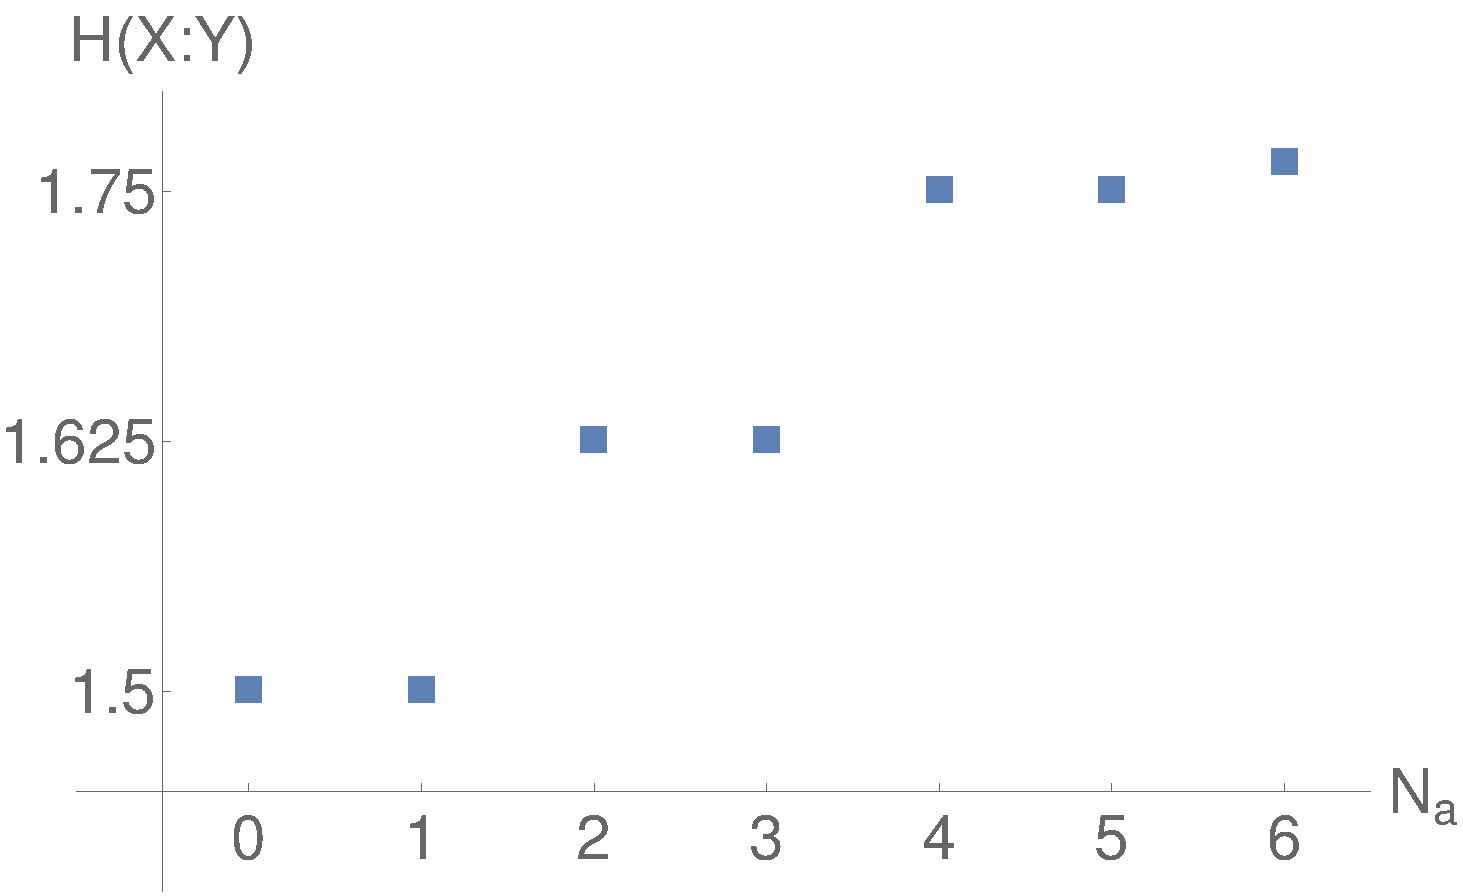
\includegraphics[width= 0.48 \textwidth]{./EntropyData.pdf}
	\caption{ Maximum mutual information $H(X:Y)$ in bits as a function of ancilla photons, $N_a$. With every additional pair of ancilla photons, we observe a gain in the mutual information of 0.125 bits. }
	\label{Mutual Information Results}
\end{figure}
We note that with every additional pair of ancilla photons, the mutual information appears to linearly approach a near-perfect measurement. If the trend continues, we expect a minimum ancilla resource of $N_a = 8$. For $N_a \ge 6$, the optimization routine becomes overwhelmed by local minima. We speculate the $N_a=6$ data point in Fig.~(\ref{Mutual Information Results}) is not a global solution for that case. We parallelized the construction of $\hat{A}(U)$ over hundreds of processes, using two Intel Xeon Phi Coprocessors. We tried BFGS, Levenberg-Marquardt, Nelder-Meade and principal axis minimization algorithms. With any of these methods, convergence still struggled for $N_a \ge 6$. In this regime, we recommend trying something other than numerical optimization.
\section{Analysis of $U$}
\label{Section on U Analysis}
The numerical results in Sec.~\ref{Section on Numerical Minimization} seem to suggest a discrete improvement as we incorporate pairs of ancilla photons into our Bell state analyzer. We now approach the problem from another other direction; we try to solve for unitary $U$ directly \textit{assuming} a near-perfect measurement.
We first define the complex variables
\begin{eqnarray}
	 A_1 = \sum\limits_{\textrm{perm}(\vec{m}^y)} U_{1,m^y_1} \dots U_{N_a,m^y_{N_a}} U_{N_a+1,m^y_{N_a+1}} U_{N_a+3,m^y_{N_a+2}} \nonumber\\
	 A_2 = \sum\limits_{\textrm{perm}(\vec{m}^y)} U_{1,m^y_1} \dots U_{N_a,m^y_{N_a}} U_{N_a+2,m^y_{N_a+1}} U_{N_a+4,m^y_{N_a+2}} \nonumber\\
	 A_3 = \sum\limits_{\textrm{perm}(\vec{m}^y)} U_{1,m^y_1} \dots U_{N_a,m^y_{N_a}} U_{N_a+1,m^y_{N_a+1}} U_{N_a+4,m^y_{N_a+2}} \nonumber\\
	 A_4 = \sum\limits_{\textrm{perm}(\vec{m}^y)} U_{1,m^y_1} \dots U_{N_a,m^y_{N_a}} U_{N_a+2,m^y_{N_a+1}} U_{N_a+3,m^y_{N_a+2}} \nonumber
\end{eqnarray}
then
\begin{eqnarray}
	& C = \frac{1}{2}\prod_{p=1}^{M} n^y_p! \nonumber \\
	& p(y|1) = C \abs{A_1 + A_2}^2\nonumber \\
	& p(y|2) = C \abs{A_1 - A_2}^2 \\
	& p(y|3) = C \abs{A_3 + A_4}^2 \nonumber\\
	& p(y|4) = C \abs{A_3 - A_4}^2 \nonumber\\
	& \sum_{x \in X} p(y|x) = C(\abs{A_1}^2 + \abs{A_2}^2 + \abs{A_3}^2 + \abs{A_4}^2 ). \nonumber
\end{eqnarray}
Because 
\begin{equation}
	0 \le p(y|x) \le 1
\end{equation}
and
\begin{equation}
	\log_2 \frac{\sum_{x^\prime} p(y|x^\prime)}{p(y|x)} \ge 0 \,,
\end{equation}
according to Eq.~(\ref{Conditional Entropy}) we need to find $U$ such that
\begin{equation}
\label{Conditional Entropy Condition}
	\forall \enspace x \enspace y , \quad p(y|x) \log_2 \frac{\sum_{x^\prime} p(y|x^\prime)}{p(y|x)} \approx 0
\end{equation}
in order to implement a near-perfect measurement. 
With some algebra, we find the condition in~(\ref{Conditional Entropy Condition}) is satisfied if and only if:
\begin{flalign}
&	\forall \quad \ket{\vec{n}^y} \mbox{,    at least one condition holds:} \nonumber \\
& (a) \enspace A_1 \approx A_2 \approx A_3 \approx A_4 \approx 0 \nonumber \\
& (b) \enspace A_1 \approx \pm A_2 \mbox{ and } A_3 \approx A_4 \approx 0 \nonumber \\ & (c) \enspace A_3 \approx \pm A_4 \mbox{ and } A_1 \approx A_2 \approx 0. \nonumber
\end{flalign}
So now, we can simply go through the output measurement states for $N_a \ge 8$, and find constraints on $U$ such that either (a),(b) or (c) is satisfied for each $\ket{\vec{n}^y}$.

We start with output states where photons are bunched into two modes; states of the form
\begin{equation}
	\ket{\vec{n}^y} = \ket{0,\dots,0,N-P,0,\dots,P,\dots,0}.
\end{equation}
up to here
\section{Discrimination of the Bell States Encoded in the Dual Rail}
Previous work in maximizing the encoding capacity of an optical quantum channel~\cite{First Paper} revealed that imposing a \textit{linear optical} encoding (Alice uses only linear optical operations to encode information into a quantum ensemble) does not prevent her from achieving the true channel capacity. But any relationship counselor will tell you that real communication generally requires a good listener; just because Alice was able to optimally compress information into the channel, does not guarantee Bob will be able to extract it. In fact, we typically observe that Bob is not able to fully discriminate an a-priori set of optical quantum states if he is restricted to a linear optical photo-counting von Neumann measurement. Formally, we define our encoded ensemble of quantum states
\begin{equation}
\{\ket{\psi_1},\ket{\psi_2},...\ket{\psi_{\abs{X}}}\},
\end{equation}  
each sent over the channel with probability $p_x$
and photo-counting measurement operators
\begin{equation}
\{ \outerproduct{\vec{n}_1}{\vec{n}_1}, \outerproduct{\vec{n}_2}{\vec{n}_2}, \dots , \outerproduct{\vec{n}_{\abs{Y}}}{\vec{n}_{\abs{Y}} } \}.
\end{equation}
A photo-counting von Neumann measurement is defined here as a unitary linear optical transformation followed by a photo-counting measurement. The probability of measuring outcome $y$ assuming state $x$ was sent will be
\begin{eqnarray}
\label{von Neumann conditional probability part 1}
\ket{\psi_x^\prime} = A(U) \ket{\psi_x} \\
\label{von Neumann conditional probability part 2}
p(y|x) = \abs{\braket{\vec{n}_y}{\psi_x^\prime}}^2.
\end{eqnarray}
Imposing this measurement scheme, the Holevo bound appears to become strict for any optical communication channel
\begin{equation}
	H(X:Y) < S(\rho).
\end{equation}
Closing the Holevo bound here is prevented by two completely separate issues. First, $\rho$ may consist of a set of non-orthogonal states. Perfectly distinguishing a set of non-orthogonal states is a general problem in quantum mechanics and a number of solutions have been proposed~\cite{Hausladen,Lloyd,Lloyd Other,Ogawa,Nagaoka,Hayashi}. Second, we are often unable to construct, even for an ensemble of orthogonal states, the necessary linear optical operator $A(U)$ to rotate all states into  non-overlapping subspaces. Here, we will focus exclusively on this second problem and attempt to improve state discrimination of a set of orthogonal quantum states. In particular, we examine the Bell states encoded in the dual-rail, defined as
\begin{eqnarray}
\rho  = \sum_{i=1}^4 \frac{1}{4} \outerproduct{\psi_i}{\psi_i} \quad \quad \quad \quad \quad \\
\ket{\psi_1} = \frac{1}{\sqrt{2}} \ket{1,0,1,0} + \frac{1}{\sqrt{2}} \ket{0,1,0,1} \\
\ket{\psi_2} = \frac{1}{\sqrt{2}} \ket{1,0,1,0} - \frac{1}{\sqrt{2}} \ket{0,1,0,1} \\
\ket{\psi_3} = \frac{1}{\sqrt{2}} \ket{1,0,0,1} + \frac{1}{\sqrt{2}} \ket{0,1,1,0} \\
\ket{\psi_4} = \frac{1}{\sqrt{2}} \ket{1,0,0,1} - \frac{1}{\sqrt{2}} \ket{0,1,1,0}
\end{eqnarray}
For this ensemble, $S(\rho)$ and $H(X)$ are both fixed at 2 bits. Numerical minimization of Eq.~(\ref{Conditional Entropy}) with Eq.~(\ref{von Neumann conditional probability part 1}) and Eq.~(\ref{von Neumann conditional probability part 2}) suggests that the optimal von Neumann measurement one can apply to this system will extract $H(X:Y) = 1.5$ bits. This is accomplished by first applying the operator $A(U)$ where
\begin{equation}
\label{First U}
U = \frac{1}{2} \begin{pmatrix} 1 & 1 & 1 & 1 \\ 1 & -1 & 1 & -1 \\ 1 & -1 & -1 & 1 \\ 1 & 1 & -1 & -1 \end{pmatrix}   
\end{equation}
and then performing a photon-counting measurement. Thus, the Bell states encoded in the dual rail form a simple, symmetric, quantum ensemble in which full state discrimination is not immediately possible. 
\section{Augmenting the System with Ancilla Resources}
\label{Augmenting Section}
Previous work in linear optical quantum computing suggests that supplementing a system with ancilla photons and modes is known to improve control over a quantum state. In particular, the gate fidelity of a measurement-assisted CNOT~\cite{KLM} acting on qubits encoded in the dual-rail improves dramatically with the proper use of ancilla resources \cite{Uskov}. So we expect to see some benefit to incorporating ancilla states here, and that is indeed the case. Our numerical experiments consisted of minimizing Eq.~(\ref{Conditional Entropy}) with Eq.~(\ref{von Neumann conditional probability part 2}) but instead of using Eq.~(\ref{von Neumann conditional probability part 1}) to define $\ket{\psi_x^\prime}$, we set
\begin{equation}
\label{Matrix Vector Product Ancilla}
\ket{\psi_x^\prime} = A(U) \ket{\psi_a} \otimes \ket{\psi_x}.
\end{equation}
In  Fig.~(\ref{Decoding Hardware Ancillas}) we present an illustration of the decoding apparatus described by Eq~(\ref{Matrix Vector Product Ancilla}). The ancilla state is defined as any Fock state constructed from $N_a$ ancilla photons and $M_a$ ancilla modes 
\begin{eqnarray}
& \ket{\psi_a} = c_1 \ket{N_a,0,\dots,0_{M_a}} + c_2 \ket{N_a-1,1,0,\dots, 0_{M_a}} + \nonumber \\ & \dots  + c_{d_{H_a}} \ket{0,0,\dots,(N_a)_{M_a}}	 \quad \quad \quad \quad
\end{eqnarray}
\begin{equation}
d_{H_a} = \frac{(N_a+M_a-1)!}{N_a ! (M_a-1)!}
\end{equation}
Because we allow photons to freely cross the boundary between computational and ancilla modes under the application of $A(U)$, the tensor product in Eq.~(\ref{Matrix Vector Product Ancilla}) falls strictly within the larger physical Hilbert space. In other words, $A(U)$ is not a square matrix. In Table~\ref{Ancilla Resources Table} we present results of numerical optimization over the unitary operator, $U$ and ancilla state $\ket{\psi_a}$.
\begin{figure}[ht]
	\centering
	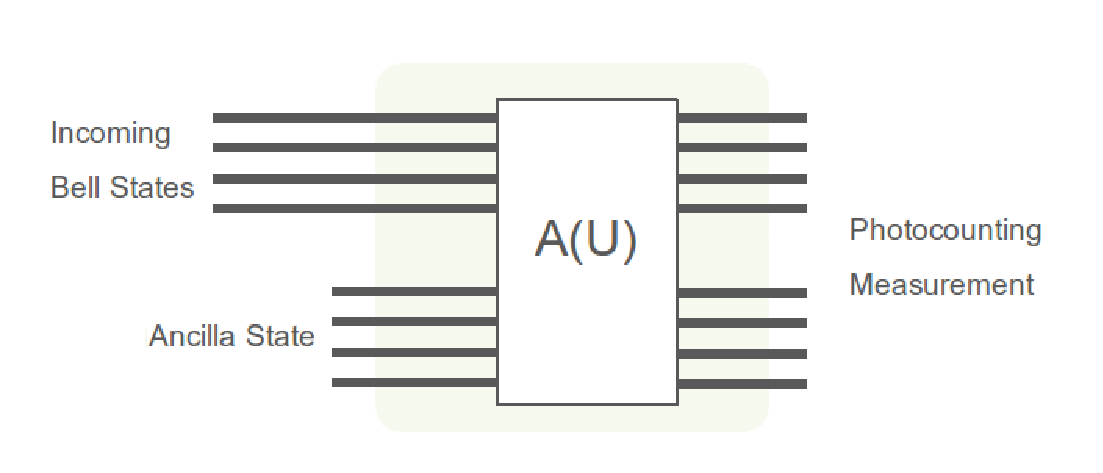
\includegraphics[width= 0.5 \textwidth]{./ancillaMeasApp.pdf}
	\caption{At the receiving end of a linear optical quantum channel, we build this measurement apparatus. Bell states arrive in the top four optical modes and we have a simple ancilla state prepared in the bottom set of modes. A linear optical transformation is applied, and then a photocounting measurement is performed.}
	\label{Decoding Hardware Ancillas}
\end{figure}
\begin {table}[H]
\begin{center}
	\begin{tabular}{l*{6}{c}r} 
		& & & &  $M_a$ \\
		&       & \vline   & 0 & 1 & 2 & 3 & 4 \\
		\cline{2-8}
		&	0    & \vline  & 1.5 & 1.5 & 1.5 & 1.5 & 1.5 \\
		&      1    & \vline & - & 1.5 & 1.5 & 1.5 & 1.5 \\
		$N_a$ & 2 & \vline & - & 1.5 & 1.625 & 1.625 & 1.625 \\
		& 3 & \vline & - & 1.5 & 1.625 & 1.625 & 1.625 \\
		& 4 & \vline & - & 1.5 & 1.625 & 1.625 & 1.75 \\
	\end{tabular}
	\caption{Results for maximization of $H(X:Y)$ in bits over the operator $A(U)$ and states $\ket{\psi_a}$ for ancilla photons $N_a$ and ancilla modes $M_a$. In a perfect measurement, $H(X:Y) \rightarrow 2$ bits.\label{Ancilla Resources Table}}
\end{center}
\end{table}
Table~\ref{Ancilla Resources Table} reports a discrete improvement in state discrimination with each additional pair of ancilla resources. We observe that all solutions converge to ancilla states $\ket{\psi_a}$ in a simple, classical state;
\begin{equation}
\ket{\psi_a} \equiv \ket{1,1,\dots,1_{M_a}}
\end{equation} In particular we present results for $N_a,M_a=0$, $N_a,M_a=2$ and $N_a, M_a= 4$. Each of these solutions represents a family of solutions which are equivalent under symmetry (e.g. invariant permutations of columns since the labeling of output modes is arbitrary). 
\newline


		$ H(X:Y) = 1.5 $ bits
		$$ \ket{\psi_a} = \ket{NULL} $$
		\begin{equation}
		\label{No Ancillas}
		U = \frac{1}{2} \begin{pmatrix} 1 & 1 & 1 & 1 \\ 1 & -1 & 1 & -1 \\ 1 & -1 & -1 & 1 \\ 1 & 1 & -1 & -1 \end{pmatrix}   
		\end{equation}
		$$or$$
		\begin{equation}
		U = \frac{1}{\sqrt 2} \begin{pmatrix} 1 & 1 & 0 & 0 \\ 0 & 0 & 1 & 1 \\ 1 & -1 & 0 & 0 \\ 0 & 0 & 1 & -1 \end{pmatrix}   
		\end{equation}

		$ H(X:Y) = 1.625 $ bits
		$$ \ket{\psi_a} = \ket{1,1} $$
		\begin{equation}
		\label{11 Ancilla}
		U = \frac{1}{2} \begin{pmatrix} 
		1 & 1 & 1 & 1 & 0 & 0 \\ 
		1 & -1 & 1 & -1 & 0 & 0 \\ 
		\frac{1}{\sqrt 2} & \frac{-1}{\sqrt 2} & \frac{-1}{\sqrt 2} & \frac{1}{\sqrt 2} & 1 & 1 \\ 
		\frac{1}{\sqrt 2} & \frac{1}{\sqrt 2} & \frac{-1}{\sqrt 2} & \frac{-1}{\sqrt 2} & i & -i \\
		\frac{1}{\sqrt 2} & \frac{1}{\sqrt 2} & \frac{-1}{\sqrt 2} & \frac{-1}{\sqrt 2} & -i & i \\
		\frac{1}{\sqrt 2} & \frac{-1}{\sqrt 2} & \frac{-1}{\sqrt 2} & \frac{1}{\sqrt 2} & -1 & -1 \\
		\end{pmatrix}   
		\end{equation}
		$$or$$
		\begin{equation}
		U = \frac{1}{2} \begin{pmatrix} 
		1 & 1 & 1 & 1 & 0 & 0 \\ 
		1 & -1 & 1 & -1 & 0 & 0 \\ 
		\frac{1}{\sqrt 2} & \frac{-1}{\sqrt 2} & \frac{-1}{\sqrt 2} & \frac{1}{\sqrt 2} & \sqrt 2 & 0 \\ 
		\frac{1}{\sqrt 2} & \frac{1}{\sqrt 2} & \frac{-1}{\sqrt 2} & \frac{-1}{\sqrt 2} & 0 & -i \sqrt 2 \\
		\frac{1}{\sqrt 2} & \frac{-1}{\sqrt 2} & \frac{-1}{\sqrt 2} & \frac{1}{\sqrt 2} & -\sqrt 2 & 0 \\
		\frac{1}{\sqrt 2} & \frac{1}{\sqrt 2} & \frac{-1}{\sqrt 2} & \frac{-1}{\sqrt 2} & 0 & i \sqrt 2 \\
		\end{pmatrix}   
		\end{equation}
		$$or$$
		\begin{equation}
		U = \frac{1}{2} \begin{pmatrix} 
		1 & 1 & 1 & 1 & 0 & 0 \\ 
		1 & -1 & 1 & -1 & 0 & 0 \\ 
		1 & 0 & -1 & 0 & 1 & 1 \\
		0 & 1 & 0 & -1 & -1 & 1 \\
		1 & 0 & -1 & 0 & -1 & -1 \\
		0 & 1 & 0 & -1 & 1 & -1 
		\end{pmatrix}   
		\end{equation}
		$ H(X:Y) = 1.75 $ bits
		\newline
		$$ \ket{\psi_a} = \ket{1,1,1,1} $$
		\newline
		\begin{equation}
		\label{1111 Ancilla}
		U = \frac{1}{2} \begin{pmatrix} 
		1 & 1 & 1 & 1 & 0 & 0 & 0 & 0 \\ 
		1 & -1 & 1 & -1 & 0 & 0 & 0 & 0 \\ 
		0 & 0 & 0 & 0 & 1 & 1 & 1 & 1 \\
		0 & 0 & 0 & 0 & 1 & -1 & 1 & -1 \\
		\frac{1}{\sqrt 2} & \frac{1}{\sqrt 2} & \frac{-1}{\sqrt 2} & \frac{-1}{\sqrt 2} & \frac{1}{\sqrt 2} & \frac{1}{\sqrt 2} & \frac{-1}{\sqrt 2} & \frac{-1}{\sqrt 2} \\ 
		\frac{1}{\sqrt 2} & \frac{-1}{\sqrt 2} & \frac{-1}{\sqrt 2} & \frac{1}{\sqrt 2} & \frac{1}{\sqrt 2} & \frac{-1}{\sqrt 2} & \frac{-1}{\sqrt 2} & \frac{1}{\sqrt 2} \\ 
		\frac{1}{\sqrt 2} & \frac{1}{\sqrt 2} & \frac{-1}{\sqrt 2} & \frac{-1}{\sqrt 2} & \frac{-1}{\sqrt 2} & \frac{-1}{\sqrt 2} & \frac{1}{\sqrt 2} & \frac{1}{\sqrt 2} \\ 
		\frac{1}{\sqrt 2} & \frac{-1}{\sqrt 2} & \frac{-1}{\sqrt 2} & \frac{1}{\sqrt 2} & \frac{-1}{\sqrt 2} & \frac{1}{\sqrt 2} & \frac{1}{\sqrt 2} & \frac{-1}{\sqrt 2} \\ 
		\end{pmatrix}   
		\end{equation}
Restating our definition of a linear optical transformation
\begin{equation}
\hat{a}^\dagger_i \rightarrow \sum_j U_{i j} \hat{a}_j^\dagger
\end{equation}
and noting that all ancilla modes are ordered \textit{before} computational modes, our results seem to suggest a general trend of spreading each pair of additional ancilla modes over four of the output modes, with discrete phase differences of $\pi$. Extrapolating these solutions, one could guess
\begin{eqnarray}
&N_a = 6, M_a = 8 : \quad \ket{\psi_a} = \ket{1,1,1,1,1,1,0,0} \nonumber \\ & \quad H(X:Y) \rightarrow 1.875 \mbox{ bits} \nonumber
\end{eqnarray}
since the three pairs of ancilla photons would then have room to spread over 12 output modes. One could further extrapolate
\begin{eqnarray}
& N_a = 8, M_a = 12 : \quad \ket{\psi_a} = \ket{1,1,1,1,1,1,1,1,0,0,0,0} \nonumber \\  & \quad H(X:Y) \rightarrow 2.0 \mbox{ bits} \nonumber
\end{eqnarray}
since the four pairs of ancilla photons have room to spread over 16 output modes. 
\newline
\newline
Unfortunately, while Eq.~(\ref{Fact 2}) allows for feasible numerical simulation of these physical systems, the large optimization space and overwhelming saturation of local minima within it prevent us from reaching a global solution. Minimization methods including BFGS, conjugate gradient descent, Levenberg-Marquardt, Nelder-Meade, and principal axis were all tried with no success. In addition, we optimized over non-unitary operators in the place of $U$ which was also unsuccessful. Pushing to simulations of this size, we recommend trying a method other than numerical optimization to find an optimal $U$.
\section{Global Quantum Channel Optimization}
In Section~\ref{Augmenting Section} we discussed using ancilla resources to improve the discrimination of states in a quantum ensemble at the receiving end of a linear optical quantum channel. We found that ancilla resources can help us to control and decode multi-photon states, though we were unable to find a protocol for perfect measurement.  Here, we finally attempt to optimize the \textit{total} capacity of a linear optical quantum channel using ancillas in the decoding phase. We allow Alice to perform a non-orthogonal encoding and we allow Bob to perform a von Neumann measurement with the help of ancilla resources, as in Fig.~\ref{Decoding Hardware Ancillas}. The full communication protocol is defined as follows;
\newline
\begin{center}
	\begin{minipage}{20em}
		(1) An entangled initial state, $\ket{\psi_1}$ is pre-distributed between Alice and Bob.
		\newline
		\newline
		(2) Alice performs some operation, $A(U_x)$ with probability $p(x)$ where $U_1 = I$ and $U_2,U_3, \dots, U_{\abs{X}}$ are unitary matrices operating only on her modes.
		\newline
		\newline
		(3) Alice's modes run to Bob, who now has possession of the entire state.
		\newline
		\newline
		(4) Bob augments the system with some pre-generated ancilla state $\ket{\psi_a}$, applies an operation to all modes $A(U_B)$, and performs a photocounting measurement.
	\end{minipage}
\end{center}
~
\newline
An illustration of the full device is presented in Fig.~(\ref{Total Quantum Channel Device}).
Formally, we want to perform a projective measurement on the ensemble of states;
\begin{equation}
\rho = \sum_{x \in X}  p(x) \outerproduct{\psi_x^\prime}{\psi_x^\prime}
\end{equation}
\begin{equation}
\ket{\psi_x^\prime} = A(U_B) A(U_x) \ket{\psi_1} \otimes \ket{\psi_a}.
\end{equation}
where according to Eq.~(\ref{Fact 1}),
\begin{equation}
A(U_B) A(U_x) = A(U_x U_B).
\end{equation}
\begin{figure}[ht]
	\centering
	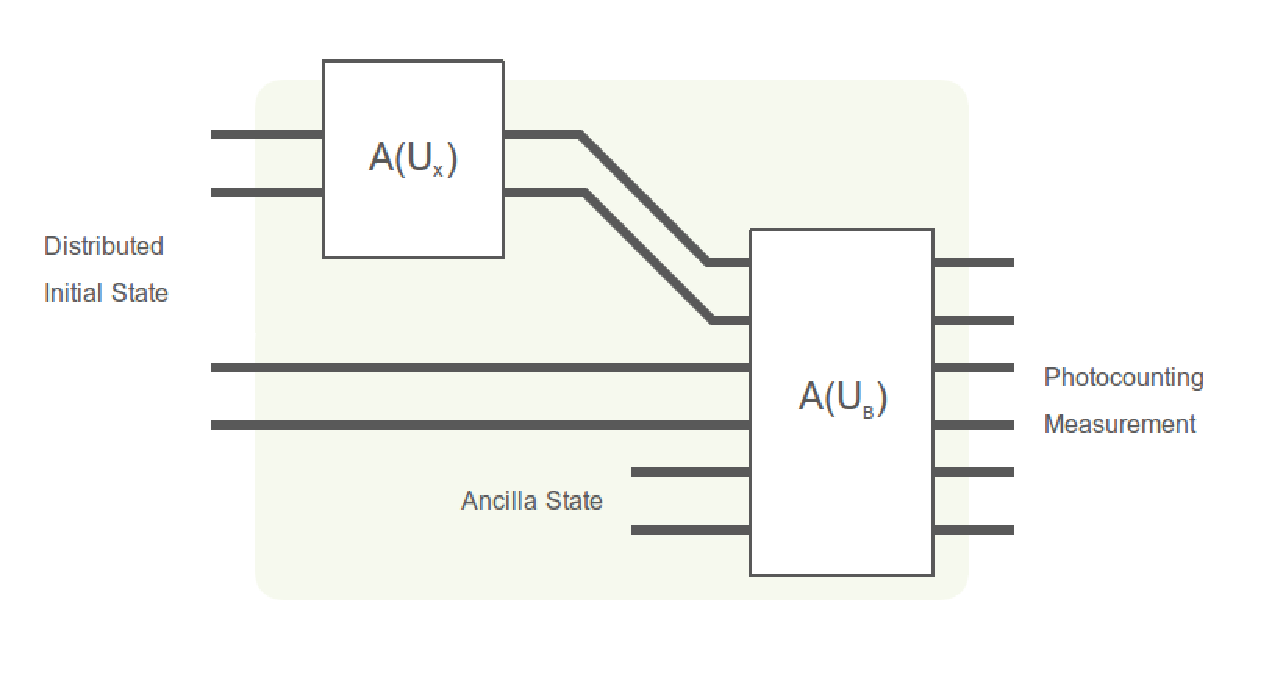
\includegraphics[width= 0.5 \textwidth]{./GlobalApparatus.pdf}
	\caption{Schematic for the total communication device. Alice and Bob each initially possess two modes. Alice acts on her modes with some operation $A(U_x)$ : $x \in X$. Alice's modes run to Bob, who augments the system with some ancilla state over two modes, applies the operation $A(U_B)$ and does a photocounting measurement.}
	\label{Total Quantum Channel Device}
\end{figure}
\newline
To quantify the success of Bob's photocounting measurement we use the mutual entropy as defined in Eq.~(\ref{Mutual Entropy Full}) and 
\begin{equation}
p(y|x) = \abs{\braket{\vec{n}_y}{\psi_x^\prime}}^2.
\end{equation}
Revisiting the key physical devices in~\cite{First Paper}, we incrementally increase the number of encoding symbols $\abs{X}$ and maximize the mutual entropy $H(X:Y)$. We then augment the systems with ancillas and attempt to close the Holevo bound. The reader should take note of our potentially confusing notation; $N_A$ and $M_A$ refer to the number of photons and modes initially in Alice's possession. $N_a$ and $M_a$ refer to the number of ancilla photons and modes that Bob augments to incoming states.
\subsection{$N=2,M=4,M_A=2$}
This system was of special interest in~\cite{First Paper} because Alice was able to achieve a maximum encoding by building an orthogonal ensemble of quantum states. We recall that in this case
\begin{eqnarray}
\abs{X} = 8 \quad \quad \quad \quad  \\
S(\rho)_{max} = \log_2 d_S = \log_2 8 = 3 \mbox{ bits}
\end{eqnarray}
\section{Conclusion}
We'll see.
\acknowledgments
I want to thank my moms, yo. This research was supported in part using high performance computing (HPC) resources and services provided by Technology Services at Tulane University, New Orleans, LA.
\begin{thebibliography}{99}

\bibitem{Reck} M. Reck, A. Zeilinger, H. J. Bernstein, and P. Bertani, Phys. Rev. Lett. {\bf 73}, 58 (1994).

\bibitem{Holevo} A. S. Holevo, Probl. Peredachi Inf. \textbf{9}, 110 (1973).	

\bibitem{First Paper} J. A. Smith, D.B. Uskov, L. Kaplan Phys. Rev. A \textbf{92}, 022324 (2015).

\bibitem{KLM}  E. Knill, R. Laflamme, G. J. Milburn, Nature (London) 409, 46 (2001).

\bibitem{Uskov} Uskov Et. Al.
Phys. Rev. A 79, 042326 (2009).

\bibitem{Adami} https://arxiv.org/abs/quant-ph/9806048

\bibitem{Review Paper} Kok Et. Al.
Rev. Mod. Phys. 79, 135 (2007).

\bibitem{Hausladen} P. Hausladen, R. Jozsa, B. Schumacher, M. Westmoreland, and W. K. Wootters, Phys. Rev. A. \textbf{54}, 1869, (1996).

\bibitem{Lloyd} S. Lloyd, V. Giovannetti, and L. Maccone, Phys. Rev. Lett. \textbf{106}, 250501 (2011).

\bibitem{Lloyd Other} V. Giovannetti, S. Lloyd, and L. Maccone, Phys. Rev. A \textbf{85}, 012302, (2012).

\bibitem{KLM2} C. R. Myers and R. Laflamme, arXiv:quant-ph/0512104 (2005).

\bibitem{Ogawa} T. Ogawa, IEEE Trans. Inf. Theory \textbf{45}, 2486 (1999).

\bibitem{Nagaoka} T. Ogawa and H. Nagaoka, IEEE Trans. Inf. Theory \textbf{53}, 2261 (2007).

\bibitem{Hayashi} M. Hayashi and H. Nagaoka, IEEE Trans. Inf. Theory \textbf{49}, 1753 (2003).

\bibitem{Lutkenhaus} N. L\"utkenhaus, J. Calsamiglia, and K.-A. Suominen, Phys. Rev. A {\bf 59}, 3295 (1999).

\bibitem{Carollo} A. Carollo and G. M. Palma, J. Mod. Opt. {\bf 49}, 1147 (2002).

\bibitem{Pavicic} M. Pavi\v{c}i\'c, Phys. Rev. Lett. {\bf 107}, 080403 (2011) (retracted).

\bibitem{Calsamiglia} J. Calsamiglia and N. L\"utkenhaus, Applied Physics B {\bf 72}, 67 (2001).

\bibitem{Ewert} F. Ewert and P. Loock, Physical Review Letters, {\bf 113}, 140403 (2014).

\bibitem{Jake Smith} J. A. Smith and L. Kaplan, arXiv: https://arxiv.org/abs/1711.01319 (2017).

\end{thebibliography}


\end{document}
